\chapter{Validação e Resultados Obtidos}
\label{chap:resultados}
O objetivo deste Capítulo é descrever todo o processo de coleta de indicadores e validação do modelo desenvolvido. Este 
Capítulo está dividido em 4 Seções.

A Seção \ref{sec:metodologia} descreve a metodologia de teste utilizada, os componentes utilizados no 
ambiente de teste e os {\it frameworks} utilizados para realizar os testes do modelo.

Na Seção \ref{sec:cenarios} são descritos os cenários definidos como casos de teste para realizar a validação do modelo.

A Seção \ref{sec:metricas} descreve quais foram as métricas utilizadas para validar o modelo.

Por fim, a Seção \ref{sec:resultados} descreve os resultados obtidos no processo de validação do modelo, as considerações e 
a importância dos resultados obtidos com o desenvolvimento do modelo.

\section{Metodologia de Teste}
\label{sec:metodologia}
A realização dos testes se deu através de um ambiente real de competição. O ambiente foi montado utilizando 4 computadores
conectadas através de um {\it switch}. As configurações dos componentes utilizados pode ser vista na tabela \ref{tab:configambiente}.

\begin{table}[!htb]

\scalefont{0.8}

\centering

\caption{Configuração dos computadores utilizados no ambiente de teste para coleta dos resultados.}.

  \begin{tabular}{|c|c|}

    \hline
    \hline
    Programa utilizado & Configuração do componente \\
    \hline
    \hline
    Time BahiaRT  & Notebook DELL Core i7, RAM-8GB, HD-1TB , Placa de vídeo - 2GB  \\
    \hline
    Time Oponente  & Notebook DELL Core i7, RAM-8GB, HD-1TB , Placa de vídeo - 2GB \\
    \hline
    Simspark  & Notebook DELL Core i7, RAM-8GB, HD-1TB , Placa de vídeo - 2GB \\
    \hline
    Roboviz & Notebook DELL Core i7, RAM-8GB, HD-1TB , Placa de vídeo - 2GB \\
    \hline
    \hline
  \end{tabular}

  \label{tab:configambiente}
\end{table}

Para realizar a validação do modelo, foi necessário instalar e configurar o Simspark e o RoboViz, que são plataformas padrões
para a simulação 3D do futebol de robôs. O servidor Simspark foi instalado em um computador e o RoboViz que é onde a simulação
do ambiente é renderizada, foi instalada em outro computador. Os outros 2 computadores, que são as máquinas clientes onde os 
binários dos times foram executados, são máquinas que possuiam apenas o sistema operacional instalado, que neste caso foi utilizado 
o {\it Ubuntu 12.04 LTS}. A arquitetura do ambiente pode ser vista através da figura \ref{fig:arquiteturaAmbiente}.

\begin{figure}[!htb]
\centering
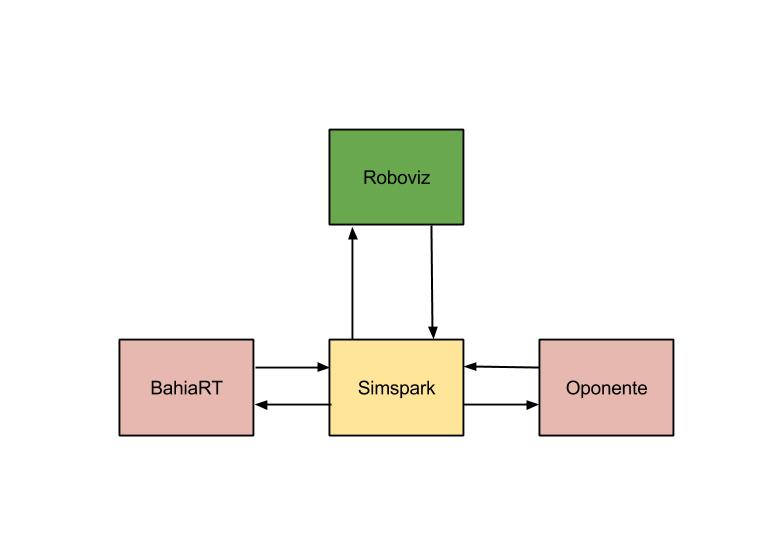
\includegraphics[scale=0.50]{figuras/ambienteTeste.jpg}
\caption{Arquitetura do ambiente de teste utilizado para coletar os resultados.} 
\label{fig:arquiteturaAmbiente}
\end{figure}
\FloatBarrier

A validação se deu através de dois processos. No primeiro processo, partidas foram realizadas utilizando $4$ times da liga de 
simulação que participaram da RoboCup 2013 e o BahiaRT:

\begin{enumerate}
 \item UTAustinVilla
 \item ITAndroids
 \item FCPortugal
 \item Apollo3D
\end{enumerate}

O objetivo do primeiro processo foi verificar a qualidade do modelo desenvolvido utilizando a predição das trajetórias dos 
obstáculos com capacidade de deliberação e a escolha da melhor trajetória para efetuar o passe com base no mapeamento dos 
obstáculos e na predição dos pontos de colisão de acordo com a velocidade e direção do agente adversário. Esta validação se 
deu através da análise de situações onde o passe ocorria verificando as métricas de avaliação que foram pré-definidas.

No segundo processo, foi utilizado uma ferramenta para automatizar testes de cenários reais de uma partida de futebol de robôs
pré-definidas utilizando agentes Dummy (agente sem capacidade de deliberação, que não se movem).

\section{Trainer3D}
Com o objetivo de automatizar os testes realizados com os agentes da simulação 3D de futebol de robôs, uma ferramenta chamada 
Trainer3D foi desenvolvida. Esta ferramenta visa facilitar a coleta dos indicadores de desempenho e também ser utilizada no processo 
de otimização dos comportamentos, como andar ou chutar.

A arquitetura do Trainer3D pode ser vista na figura \ref{fig:trainer3d}.

\begin{figure}[!htb]
\centering
\scalefont{1.0}
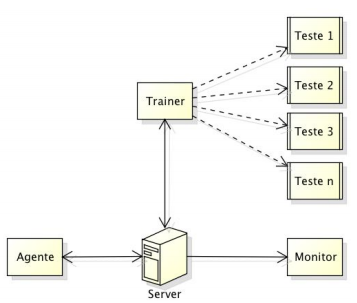
\includegraphics[scale=0.8]{figuras/trainer3d.png}
\caption{Arquitetura da ferramenta Trainer3D.} 
\label{fig:trainer3d}
\end{figure}
\FloatBarrier

Quando o Trainer3D é instanciado, ele gera uma comunicação com o servidor SimSpark através de um socket com protocolo TCP/IP que capta as 
mensagens do estado do agente, bola e campo. A partir da comunicação do trainer com o servidor, as mensagens que o servidor envia são 
quebradas em tokens que contém informações do ambiente que está sendo simulado e que são renderizadas pelo RoboViz.

Além de captar as mensagens do servidor, o trainer também possui a característica de mudar o estado do ambiente. Para mudar o estado do ambiente, 
mensagens específicas são enviadas ao servidor. Cada mensagem para alterar o estado de um objeto no ambiente deve conter um identificador que 
indica qual objeto deve ser atualizado.

As mensagens que o Trainer3D recebe possuem informações como posicionamento da bola e dos agentes que estão no campo. Com 
essas informações, é possível fazer uma análise de como o agente está atuando, se está caído, qual a velocidade média de deslocamento 
do agente, se a bola foi chutada, e outras informações.

Com o desenvolvimento da ferramenta, foi possível coletar os resultados dos testes realizados com os cenários pré-definidos de forma 
automatizada, sem a necessidade de interfer\^encia humana.

\section{Cenários de Teste}
\label{sec:cenarios}
O objetivo dos cenários de teste foi diversificar as situações em que o agente (ou robô) pudesse utilizar o modelo para encontrar
a melhor trajetória para realizar o seu objetivo, que no caso foi definido como efetuar um passe para um outro agente aliado. Um 
passe no futebol é fazer com que um agente $A$ chute a bola para um agente $B$, de modo que o agente $B$ possa receber a bola em 
uma posição estratégica.

Os cenários foram divididos em níveis de dificuldade. O nível de dificuldade foi definido como a quantidade de agentes oponentes, 
que são considerados obstáculos móveis que podem comprometer a realização do objetivo do agente que vai efetuar o passe da bola. Os 
níveis foram mapeados de acordo com a tabela \ref{tab:niveisDificuldade}.

\begin{table}[!htb]

\scalefont{0.8}

\centering

\caption{Nível A é considerado fácil, o B é considerado moderado, C é considerado difícil, e o D é considerado muito difícil.}

  \begin{tabular}{|c|c|}
    \hline
    Quantidade de oponentes & Nível de dificuldade \\ \hline
    2  & A \\ \hline
    3  & B \\ \hline
    4  & C \\ \hline
    4+ & D \\ \hline
  \end{tabular}

  \label{tab:niveisDificuldade}
\end{table}

Na figura \ref{fig:cenario}, são demonstradas as situações escolhidas para realizar os testes utilizando agentes oponentes que não se movem. 
Nestas situações, o objetivo foi verificar se o agente estava escolhendo a melhor trajetória para efetuar o passe e o 
executando corretamente.

\begin{figure}[!htb]
\centering
\scalefont{1.0}
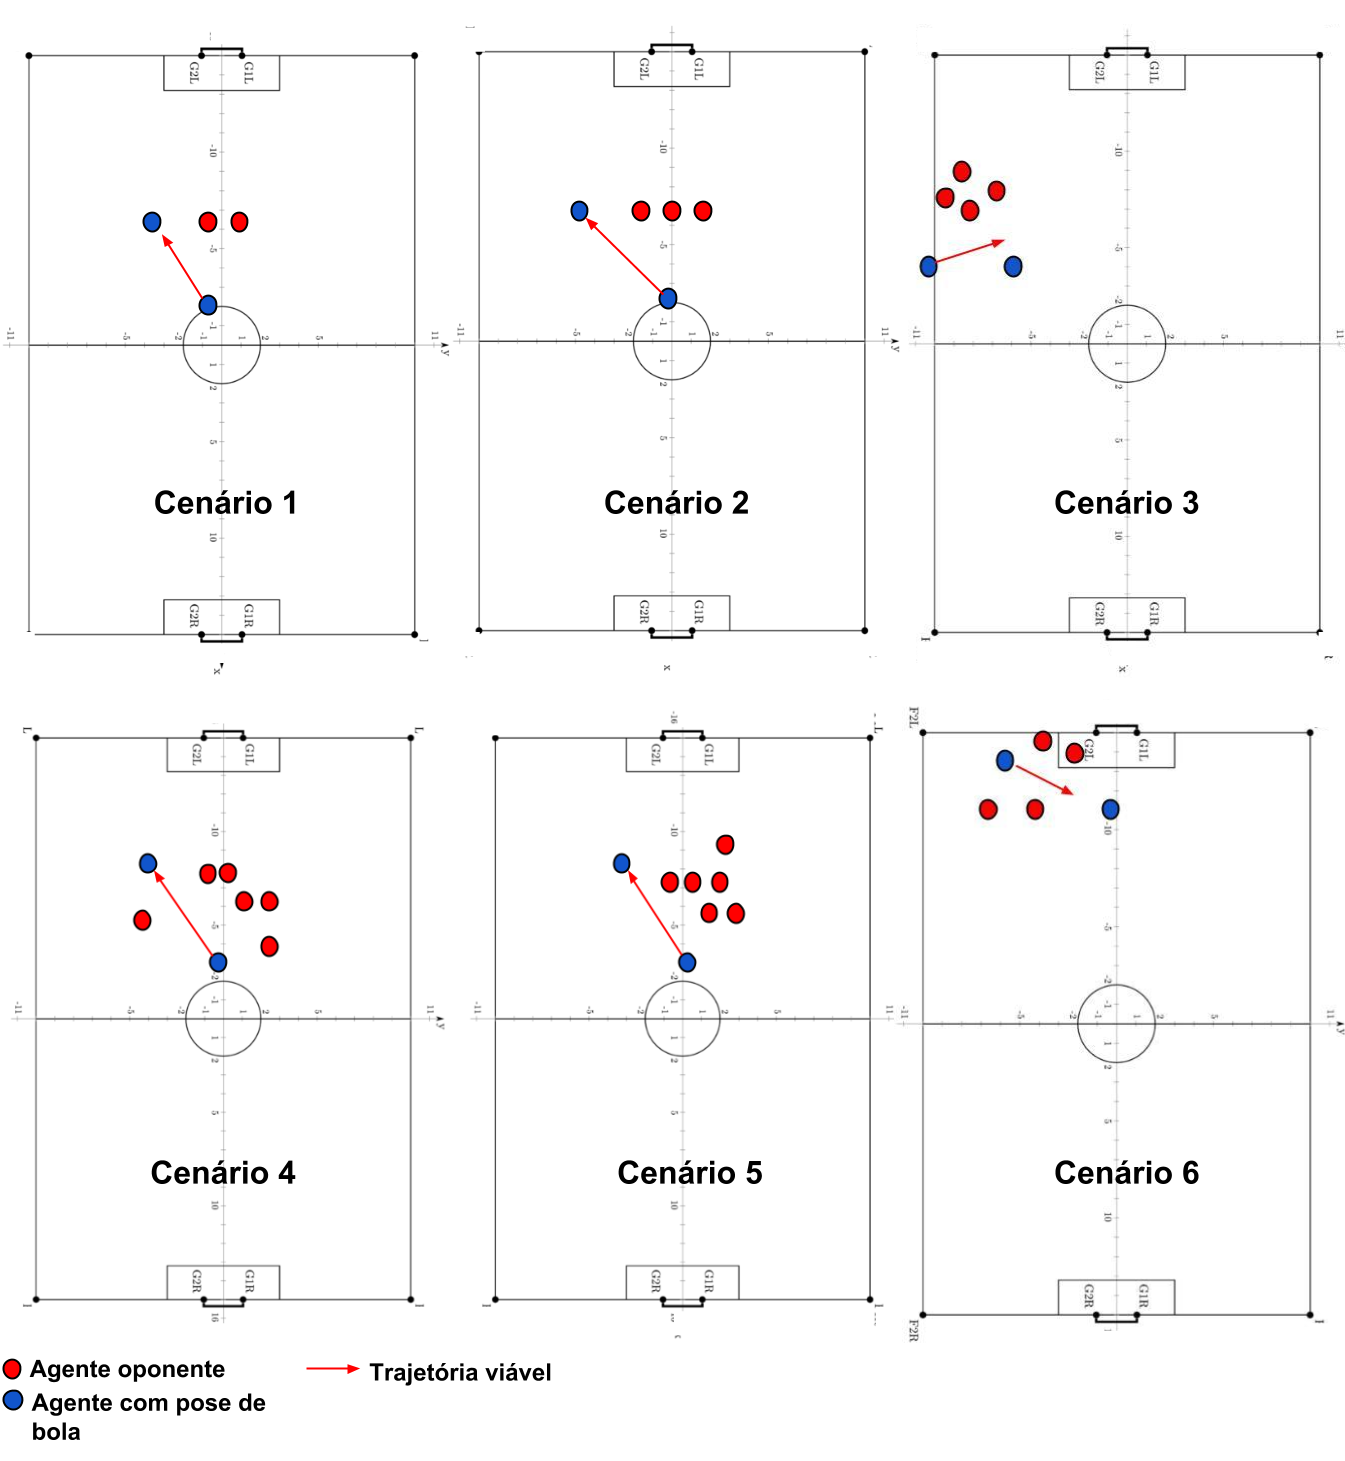
\includegraphics[scale=0.3]{figuras/Cenario.png}
\caption{Cenários de situações de um jogo real de futebol onde um agente tem a possibilidade de efetuar um passe para outro agente 
aliado em uma posição estratégica.} 
\label{fig:cenario}
\end{figure}
\FloatBarrier

\section{Métricas de Avaliação}
\label{sec:metricas}
Os indicadores escolhidos para validar o modelo proposto foram mapeados levando em consideração aspectos que não são 
influênciados por problemas que não estão dentro do contexto do problema em questão, que é o planejamento de trajetória em tempo 
real.

Para o primeiro processo de validação, foram definidas $5$ métricas:

\begin{enumerate}
    \item Quantidade total de passes
    \item Quantidade de passes corretos em kickin
    \item Quantidade de passes corretos em goal\_kik
    \item Quantidade de passes corretos em play\_on
    \item Quantidade de passes errados
\end{enumerate}

Para o segundo processo de validação, a métrica utilizada para validar o modelo foi a escolha da trajetória com base no 
cenário de teste executado.

Os testes executados que não estavam de acordo com a especificação da metodologia adotada, foram desconsiderados. O objetivo foi 
ter resultados bem definidos, que não foram afetados por outros problemas que ainda são lacunas a serem resolvidas em 
trabalhos posteriores.

\section{Resultados} 
\label{resultados}
O objetivo dessa seção é descrever os resultados obtidos no processo de validação através do ambiente real de jogo e de cenários 
pré-definidos. Todos os testes foram realizados utilizando o ambiente descrito na figura \ref{fig:arquiteturaAmbiente}. A análise 
dos resultados do primeiro processo de validação foi feita através do log gerado da partida pelo RoboViz, onde é possível reproduzir
todo o jogo, parando, voltando e adiantando quando necessário.

\subsection{Resultados de partidas utilizando cenário de jogo real}

Inicialmente foram realizadas $10$ partidas com alguns times da liga de simulação com duração de $10$ minutos cada partida. Os 
resultados preliminares demonstrados na tabela \ref{tab:resultado3}, mostraram que em mais de $40\%$ das tentativas de passe, 
onde o agente tinha condições favoráveis, o mesmo era cancelado por conta da demora para se posicionar e realizar o chute, e da
aproximação do agente adversário. Em alguns testes, quando o chute da bola alcançava uma dist\^ancia muito curta, os agentes 
oponentes conseguiam ter a pose de bola.

\begin{table}[H]

\scalefont{0.8}
\centering
\caption{Tabela com o resultados preliminares dos testes realizado com times da liga de simulação 3D}.

\begin{tabular}{|p{3cm}|c|c|c|c|c|}
    \hline
    Time & Apollo3D & UTAustinVilla & FCPortugal & ITAndroids \\ \hline
    Quantidade de passes	   				  & 57      & 54       & 35      & 105     \\ \hline
    Quantidade de passes corretos 				  & 8.77\%  & 18.52\%  & 31.43\% & 38.10\% \\ \hline
    Quantidade de passes que terminaram em gol 		  & 0.00\%  & 0.00\%   & 0.00\%  & 2.86\%  \\ \hline
    Quantidade de passes errados que terminaram em gol		  & 3.51\%  & 0.00\%   & 0.00\%  & 0.00\%  \\ \hline
    Quantidade de passes errados com pose de bola do adversário & 8.77\%  & 11.11\%  & 15.24\% & 15.24\% \\ \hline
    Quantidade de passes desistidos 				  & 78.95\% & 70.37\%  & 43.81\% & 43.81\% \\ \hline
  \end{tabular}

  \label{tab:resultado3}
\end{table}

Após a conclusão do projeto, foram realizadas $5$ partidas com duração de $10$ minutos para cada time. Os resultados obtidos 
no processo de validação final utilizando o cenário de jogo real demonstraram uma melhora significativa na quantidade de passes 
realizados com sucesso. Na tabela \ref{tab:resultado2} são demonstrados os resultados obtidos.  

\begin{table}[H]

\scalefont{0.8}
\centering
\caption{Tabela com o resultado dos testes realizado com times da liga de simulação 3D}.

  \begin{tabular}{|p{3cm}|c|c|c|c|c|}
    \hline
    Time & Mithras3d & UTAustinVilla & RoboCanes & Hfutengine \\ \hline
    Quantidade total de passes				& 15	 & 4   & 6  &  4\\ \hline       
    Quantidade de passes corretos em kickin	  	& 0      & 2   & 4  &  2\\ \hline
    Quantidade de passes corretos em goal\_kick 	& 0      & 2   & 2  &  	0\\ \hline
    Quantidade de passes corretos em play\_on 	  	& 15     & 0   & 0  &  	2\\ \hline
    Quantidade de passes errados	  		& 0	 & 0   & 0  &  	0\\ \hline
    
  \end{tabular}

  \label{tab:resultado2}
\end{table}

Os resultados obtidos demonstraram que em situações de bola parada, \textit{kickin}, \textit{goal\_kick}, 
onde o agente possui mais tempo para se posicionar e chutar a bola, os passes tiveram 100\% de acerto. Porém, em situações onde 
a bola está em jogo, \textit{play\_on}, sendo disputada por outros jogadores, ficou evidente que o principal fator responsável 
por permitir que o agente consiga efetuar mais passes é a velocidade com que o chute é executado. Contra o time Mithras3d, onde 
seus agentes possuia movimentação mais lenta, o agente conseguiu efetuar mais passes em modo \textit{play\_on}. Porém, contra o 
RoboCanes e UTAustinVilla, o agente não conseguiu efetuar passes em modo \textit{play\_on} devido a velocidade rápida da movimentação 
dos seus agentes. Ainda assim, nas situações de bola parada, os passes realizados permitiram ao BahiaRT obter vantagem estratégica.

\begin{table}[H]

\scalefont{0.8}
\centering
\caption{Tabela com o resultado das partidas realizadas no processo de validação}.

  \begin{tabular}{|p{3cm}|c|c|c|c|c|c|c|c|c|}
    \hline
    Time 		& Vitórias & Empates  & Derrotas & Gols Marcados & Gols Sofridos & Saldo de Gols \\ \hline
    Mithras3d	  	& 5        & 0   & 0  & 30  &  0 & 30  \\ \hline
    UTAustinVilla 	& 0        & 0   & 5  &  0  & 13 & -13 \\ \hline
    RoboCanes 	  	& 1        & 3   & 1  &  4  & 4  & 0 	\\ \hline
    Hfutengine	  	& 5	   & 0   & 0  & 22  & 0  & 22  \\ \hline
    
  \end{tabular}

  \label{tab:tabelajogos}
\end{table}

Na tabela \ref{tab:tabelajogos} são mostrados os resultados das partidas realizadas no processo de validação. Com o modelo de passe, 
o BahiaRT conseguiu obter maior aproveitamento, vencendo a maioria das partidas realizadas. Nos jogos realizados contra o time UTAustinVilla, 
o BahiaRT perdeu todas as partidas por conta do super chute realizado pelo time oponente. Tais gols não puderam ser evitados, pois foram realizados 
em situações de bola parada, nas laterais e no meio de campo. Já contra o Mithras3d e Hfutengine, o BahiaRT conseguiu obter maior aproveitamento de gols. 
Por último, o RoboCanes foi o time mais equilibrado, com forte marcação na defesa, dificultando as chances de passe e marcação de gols.

\subsection{Resultados utilizando cenários pré-definidos}
Os resultados obtidos no segundo processo de validação, onde foram realizados $20$ testes com situações pré-definidas 
demonstraram a eficácia do modelo desenvolvido em ambientes estáticos. Em todos os casos, o agente escolheu a melhor 
trajetória para efetuar o passe com base na segurança da trajetória e no posicionamento do agente aliado que recebeu o passe. 
Além disso, ficou evidente que independente do nível de dificuldade descrito na tabela \ref{tab:niveisDificuldade}, o 
agente consegue mapear e escolher a melhor trajetória.

Para demonstrar os resultados, foram plotados os pontos em que os agentes aliados e oponentes estavam posicionados e a
trajetória escolhida para realizar o passe utilizando o modelo desenvolvido. Foram plotadas \`as trajetórias na cor verde através 
de retas entre os pontos inicial e final, aliados com pontos em preto e oponentes em cor vermelha. Os resultados podem ser 
vistos nas figuras \ref{fig:cenario123} e \ref{fig:cenario456}.

%FIGURA COM OS RESULTADOS DOS AGENTES DUMMY

\begin{figure}[H]
\centering
\scalefont{1.0}
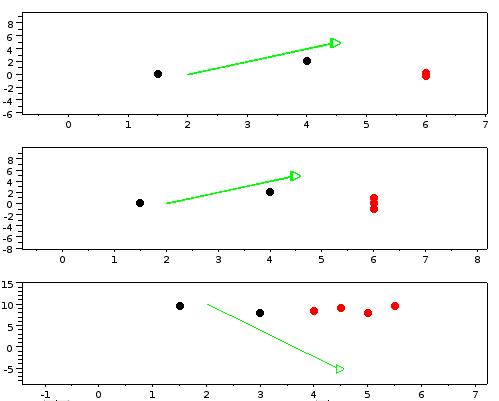
\includegraphics[scale=0.6]{figuras/cenario123.png}
\caption{Resultados dos testes realizados com agentes Dummy nos cenários pre-definidos.} 
\label{fig:cenario123}
\end{figure}
\FloatBarrier


\begin{figure}[H]
\centering
\scalefont{1.0}
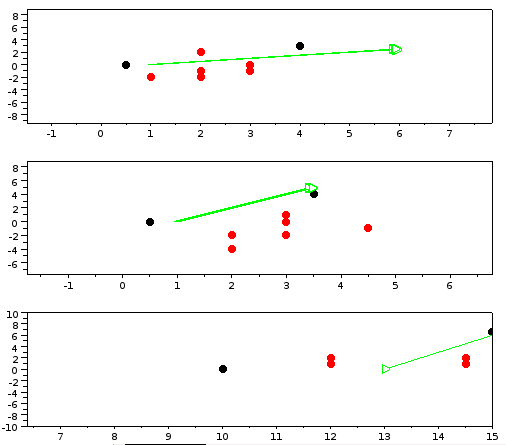
\includegraphics[scale=0.6]{figuras/cenario456.png}
\caption{Resultados dos testes realizados com agentes Dummy nos cenários pre-definidos.} 
\label{fig:cenario456}
\end{figure}
\FloatBarrier
